%%\documentclass[a4paper,11pt]{article}
\documentclass[11pt]{article}

\usepackage[left=2.5cm, right=2cm, top=0.6cm, bottom=2cm, includehead, includefoot]{geometry}
\usepackage[utf8]{inputenc}
\usepackage[T1]{fontenc}
\usepackage{titlesec}
\usepackage{enumitem}
\usepackage{graphicx}
\usepackage{amsmath}
\usepackage{amsfonts}
\usepackage{amssymb}
\usepackage{parskip}
\usepackage{float}
\usepackage{setspace}
\usepackage{fancyhdr}
\usepackage{needspace}
\usepackage{etoolbox}

\pagestyle{fancy}
\fancyhf{}
\setlength{\headheight}{63pt}
\setlength{\headsep}{10pt}
\fancyhead[L]{}
\fancyhead[R]{}
\fancyhead[C]{
\includegraphics[width=\textwidth]{picture/logo.pdf}}
\renewcommand{\headrulewidth}{0pt}
\fancyfoot[C]{\thepage}
\setlength{\footskip}{18pt}

\setstretch{1.12}
\setlength{\parskip}{0.65em}
\setlist[itemize]{leftmargin=1.35cm, itemsep=0.45em, topsep=0.35em}
\setlist[enumerate]{leftmargin=1.35cm, itemsep=0.45em, topsep=0.35em}

\titleformat{\section}{\normalfont\Large\bfseries}{\thesection}{1em}{}
\titleformat{\subsection}{\normalfont\large\bfseries}{\thesubsection}{1em}{}
\preto{\subsection}{\Needspace{10\baselineskip}}
\preto{\subsubsection}{\Needspace{8\baselineskip}}

\title{Informe del Proyecto}
\raggedbottom

\begin{document}

\renewcommand{\figurename}{Figura}
\renewcommand{\thesection}{\Roman{section}}
\begin{center}
    \textbf{\underline{\normalsize APE 1}}
\end{center}

\section{PORTADA}

\begin{tabbing}
    \textbf{Unidad de Organización Curricular:}\hspace{1cm} \= \kill
    \textbf{Tema:} \> Ecualizador Modular para Procesamiento de Imágenes \\[0.25em]
    \textbf{Carrera:} \> Ingeniería de Software \\[0.25em]
    \textbf{Unidad de Organización Curricular:} \> PROFESIONAL \\[0.25em]
    \textbf{Nivel y Paralelo:} \> Séptimo semestre A \\[0.25em]
    \textbf{Alumnos participantes:} \> Paul Velastegui \\
    \> David Manjarres \\[0.25em]
    \textbf{Asignatura:} \> Gestión de Proyectos \\[0.25em]
    \textbf{Docente:} \> Ing. Rubén Nogales, Mg.
\end{tabbing}

\section{INFORME DE GUÍA PRÁCTICA}
\renewcommand{\thesection}{\arabic{section}}

\subsection{Objetivos}
\textbf{General:}
\begin{itemize}
    \item Aplicar un flujo de preprocesamiento de imágenes bajo arquitectura MVVM que permita la mejora del contraste mediante normalización min-max por canal, la conversión a escala de grises, la compresión espacial por bloques y la segmentación binaria por umbralización, evaluando el sistema con imágenes de alta complejidad espectral.
\end{itemize}

\textbf{Específicos:}
\begin{itemize}
    \item Analizar la distribución de intensidades de la imagen original mediante histogramas por canal R, G y B, antes y después de aplicar la normalización min-max, para evidenciar la expansión del contraste.
    \item Implementar la normalización min-max de forma independiente sobre cada canal RGB usando NumPy y OpenCV, reconstruyendo la imagen base a partir de los tres canales normalizados.
    \item Obtener la imagen comprimida en escala de grises mediante promediado por bloques de $N \times N$ y su versión binarizada, observando el efecto de los controles de tamaño de bloque y umbral sobre el resultado final.
\end{itemize}

\subsection{Modalidad}
\begin{tabbing}
    \hspace{1cm} \= Presencial.
\end{tabbing}

\subsection{Tiempo de duración}
\begin{tabbing}
    \hspace{1cm} \= \textbf{Presenciales:} \= 8 \\
    \hspace{1cm} \= \textbf{No presenciales:} \= 0
\end{tabbing}

\subsection{Instrucciones}
\begin{enumerate}
    \item Seleccionar una imagen de entrada para realizar el procesamiento.
    \item Normalizar la imagen y observar los cambios generados en su representación visual.
    \item Visualizar la imagen desde sus canales de color para comparar la información presente en cada uno.
    \item Comprimir la imagen en escala de grises mediante bloques de reducción.
    \item Aplicar binarización por umbral para obtener una imagen compuesta únicamente por valores claros y oscuros.
\end{enumerate}

\subsection{Listado de equipos, materiales y recursos}
Listado de equipos y materiales generales empleados en la guía práctica:
\begin{itemize}
    \item Computador.
    \item Imagen de prueba de alta complejidad espectral (región de formación estelar W51).
    \item Entorno de desarrollo Python 3 con PySide6, OpenCV y NumPy.
    \item Internet.
    \item Material disponible en el aula virtual de la asignatura.
    \item Herramientas que permitan generar documentos en formato PDF.
\end{itemize}

\textbf{TAC (Tecnologías para el Aprendizaje y Conocimiento) empleados en la guía práctica:}

$\square$ Plataformas educativas \\
$\square$ Simuladores y laboratorios virtuales \\
$\blacksquare$ Aplicaciones educativas \\
$\square$ Recursos audiovisuales \\
$\square$ Gamificación \\
$\blacksquare$ Inteligencia Artificial \\
Otros (Especifique): \underline{\hspace{5cm}}

\subsection{Actividades por desarrollar}
\begin{enumerate}
    \item Cargar la imagen de la región W51 y generar los histogramas originales por canal.
    \item Aplicar la normalización por canal y generar los histogramas normalizados.
    \item Obtener la imagen en escala de grises, comprimirla por bloques y aplicar la binarización por umbral.
    \item Comparar la imagen original, la normalizada, la comprimida en escala de grises y la binarizada.
\end{enumerate}

\subsection{Material y Caso de Estudio}

En esta sección se presenta la imagen seleccionada como caso de estudio, justificando su elección en función de su complejidad espectral y la correspondencia con los algoritmos implementados en la herramienta.

\subsubsection{Región de formación estelar W51 (James Webb Space Telescope, 2025)}

Esta imagen corresponde a una de las observaciones más recientes y de mayor resolución de la región de formación estelar W51, capturada por el Telescopio Espacial James Webb (JWST). La adquisición de los datos fue realizada por investigadores de la Universidad de Florida, con contribuciones de NASA, ESA y CSA, así como del equipo Yoo \& Ginsburg, mientras que el procesamiento estuvo a cargo de A.~Pagan (STScI) \cite{jwst_w51}. El uso de instrumentos de infrarrojo cercano (NIRCam) y medio (MIRI) permite obtener una representación detallada de estructuras que no son visibles en el espectro óptico.

El empleo de observaciones en el rango infrarrojo resulta fundamental en el estudio de regiones de formación estelar, ya que estas longitudes de onda pueden atravesar densas nubes de polvo interestelar que bloquean la luz visible. Esto posibilita la detección directa de estrellas jóvenes que permanecen ocultas dentro de dichas nubes, aportando información clave sobre las etapas tempranas de evolución estelar y la dinámica del medio interestelar \cite{jwst_w51}.

Las imágenes obtenidas revelan estructuras complejas, incluyendo nubes de gas ionizado, filamentos de polvo y chorros de material expulsado por estrellas jóvenes. La aplicación de técnicas de procesamiento, como la normalización \textit{min-max}, permite resaltar regiones de baja intensidad como estrellas ``escondidas'' detrás del gas más denso y mejorar el contraste general de la imagen. Este tipo de análisis evidencia la utilidad de herramientas computacionales para extraer información espectral y espacial relevante, facilitando una interpretación más precisa de los fenómenos observados.

\begin{figure}[!htbp]
    \centering
    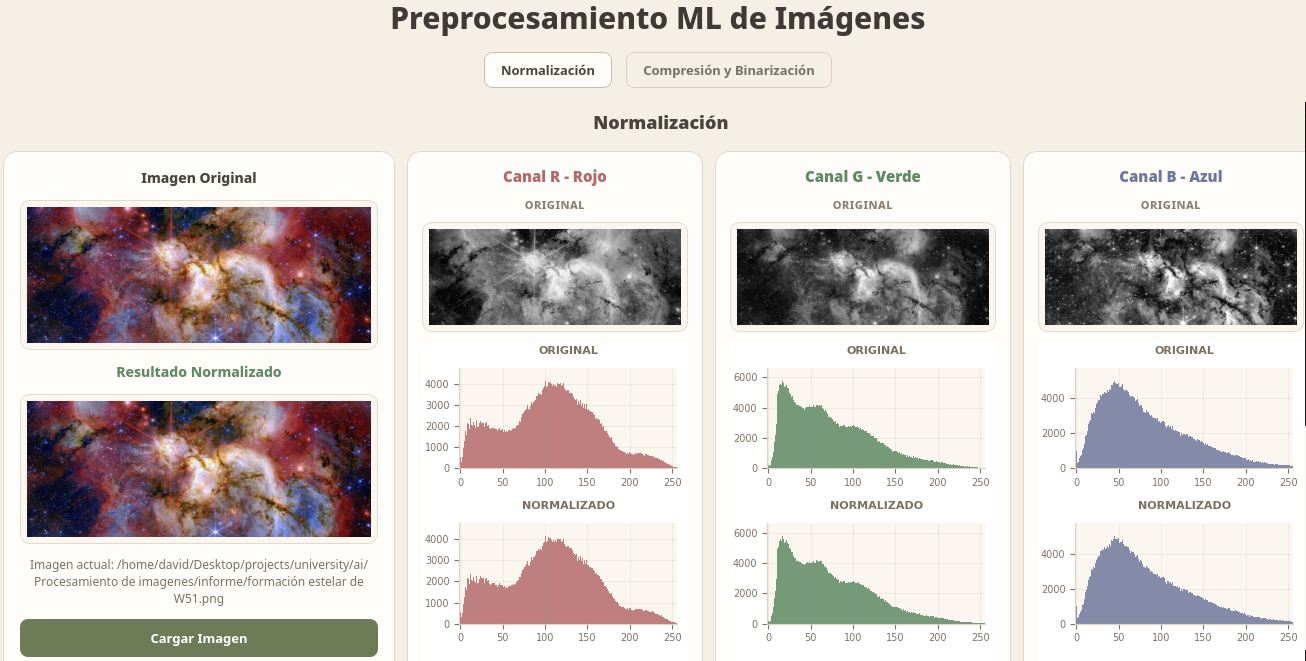
\includegraphics[width=0.92\textwidth]{img/app_interfaz_w51.png} % captura de la app con W51 cargada (pantalla de Normalización)
    \caption{Vista superior de la interfaz de la herramienta con la imagen W51 cargada: panel de imagen original (izquierda) y tarjetas de los canales R, G y B con sus histogramas originales.}
    \label{fig:app_interfaz}
    \vspace{2pt}
    {\footnotesize Fuente: Elaboración propia.}
\end{figure}

\begin{figure}[!htbp]
    \centering
    \includegraphics[width=0.82\textwidth]{"formación estelar de W51.png"}
    \caption{Región de formación estelar W51 capturada por el JWST.}
    \label{fig:w51}
    \vspace{2pt}
    {\footnotesize Fuente: NASA, ESA, CSA, Yoo \& Ginsburg (UF); procesamiento: A.~Pagan (STScI) \cite{jwst_w51}.}
\end{figure}

\subsection{Resultados obtenidos}

En esta sección se documenta el procedimiento aplicado sobre la imagen de la región estelar W51. Se parte de la imagen original, se analizan sus histogramas por canal, se aplica la normalización, se obtiene la imagen normalizada junto con su versión en escala de grises y binaria, y finalmente se comparan los resultados.

\subsubsection{Imagen original utilizada}

La imagen empleada corresponde a la región de formación estelar W51, obtenida por el JWST en el infrarrojo cercano y medio. Esta imagen constituye el punto de partida del procesamiento. Su características más relevante para los fines de esta práctica es que presenta amplias zonas de alto brillo (nubes de gas ionizado) junto con regiones de muy baja intensidad donde se encuentran las estrellas en formación, cubiertas por polvo. Esto genera un histograma comprimido con concentración en valores intermedios y una diferencia de contraste local reducida, lo cual la convierte en un caso de estudio ideal para la expansión min-max.

\begin{figure}[!htbp]
    \centering
    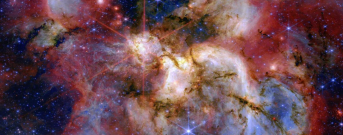
\includegraphics[width=0.55\textwidth]{img/w51_original_panel.png}
    \caption{Panel de imagen original en la herramienta, mostrando la región W51 tal como fue cargada, sin ningún procesamiento aplicado.}
    \label{fig:original_panel}
    \vspace{2pt}
    {\footnotesize Fuente: Elaboración propia.}
\end{figure}

\subsubsection{Análisis de histogramas originales}

Antes de aplicar cualquier transformación, la herramienta genera automáticamente los histogramas de los tres canales RGB de la imagen original para cada canal por separado. Estos histogramas muestran la distribución real de intensidades tal como aparece en la imagen base. El eje horizontal representa el valor de intensidad del píxel (de 0 a 255) y el eje vertical indica la cantidad de píxeles con ese valor.

\begin{figure}[!htbp]
    \centering
    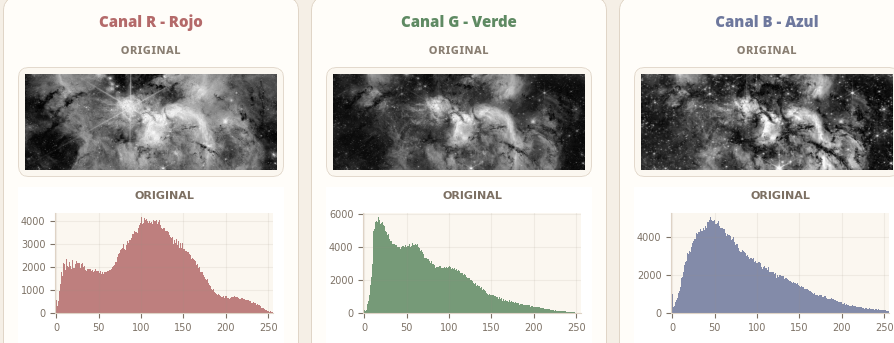
\includegraphics[width=0.92\textwidth]{img/histogramas_originales_rgb.png}
    \caption{Histogramas originales de los canales R, G y B de la imagen W51, generados por la herramienta antes de aplicar ninguna transformación.}
    \label{fig:hist_orig}
    \vspace{2pt}
    {\footnotesize Fuente: Elaboración propia.}
\end{figure}

Los tres canales de la imagen infrarroja del JWST presentan distribuciones distintas. El canal rojo concentra sus valores en el rango de 0 a 250, con mayor densidad entre 50 y 180, correspondiente a la emisión general del gas caliente. El canal verde presenta su concentración entre 0 y 100, con una caída pronunciada a partir de los 50 niveles de intensidad, reflejando el contraste entre el polvo frío y el gas ionizado. El canal azul muestra una distribución similar al verde pero con la masa principal de píxeles concentrada entre 0 y 80, correspondiente a estructuras más frías o alejadas del frente de ionización.

\subsubsection{Normalización por canales}

La normalización por canal es una técnica de preprocesamiento que redistribuye los valores de intensidad dentro de un rango seleccionado manualmente, llevándolo a ocupar el espacio completo de 0 a 255. Su utilidad concreta consiste en que, si la información útil de un canal se concentra en un rango estrecho, al estirar ese rango se amplían las diferencias de brillo entre estructuras y se mejora el contraste visual \cite{gonzalez}.

La fórmula aplicada corresponde a la normalización min-max:
\begin{equation}
    p_{nuevo} = \frac{p - p_{\min}}{p_{\max} - p_{\min}} \times 255
    \label{eq:normalizacion}
\end{equation}
Donde $p$ es el valor original del píxel, $p_{\min}$ y $p_{\max}$ son los límites inferior y superior del rango elegido, y $p_{nuevo}$ es el valor resultante. Los píxeles por debajo de $p_{\min}$ se fijan en 0 y los que superan $p_{\max}$ se fijan en 255. La implementación en \texttt{modelo.py} aplica esta fórmula de forma independiente sobre cada canal, procesando el arreglo NumPy completo sin iterar sobre píxeles individuales.

Los rangos aplicados a cada canal para la imagen W51 son los siguientes:

\textbf{Canal rojo: $p_{\min} = 36$, $p_{\max} = 170$.} El canal rojo presenta el rango más amplio entre los tres canales. Al excluir los 36 niveles inferiores (fondo oscuro del espacio) y recortar la saturación a partir de 170, se evita que las zonas de mayor brillo del gas ionizado dominen la normalización, preservando la información de contraste en las regiones intermedias donde se encuentran las estructuras estelares en formación.

\textbf{Canal verde: $p_{\min} = 88$, $p_{\max} = 255$.} El canal verde concentra su información útil a partir de los 88 niveles de intensidad. Al fijar el mínimo en ese punto, se eliminan los píxeles oscuros del fondo que no aportan información relevante y se expande el rango efectivo hacia el límite superior, logrando el mayor incremento de contraste en bordes y filamentos de polvo.

\textbf{Canal azul: $p_{\min} = 35$, $p_{\max} = 255$.} El canal azul presenta una distribución concentrada en valores bajos. Al establecer el mínimo en 35 se descartan únicamente los niveles más oscuros del fondo, y al mantener el máximo en 255 se aprovecha toda la información disponible en el canal, ampliando la representación de las estructuras más frías de la región.

Una vez normalizados los tres canales de forma independiente, se reconstruye la imagen RGB normalizada ($RGB_{norm}$) apilando los canales resultantes mediante \texttt{np.stack}. Esta imagen sirve como entrada única y coherente para los procesos de la segunda etapa.

\subsubsection{Histogramas normalizados}

Tras aplicar la normalización se generan automáticamente los histogramas correspondientes a cada canal, que la herramienta muestra en las tarjetas de canal (sección ``NORMALIZADO'') junto al histograma original, permitiendo una comparación directa.

\begin{figure}[!htbp]
    \centering
    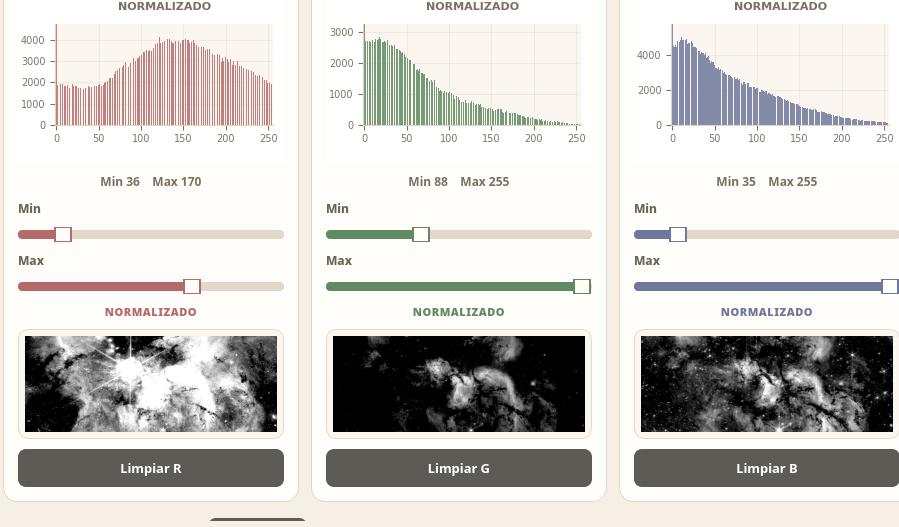
\includegraphics[width=0.92\textwidth]{img/histogramas_normalizados_rgb.png}
    \caption{Histogramas normalizados de los canales R ($p_{\min}=36$, $p_{\max}=170$), G ($p_{\min}=88$, $p_{\max}=255$) y B ($p_{\min}=35$, $p_{\max}=255$) tras aplicar la expansión min-max.}
    \label{fig:hist_norm}
    \vspace{2pt}
    {\footnotesize Fuente: Elaboración propia.}
\end{figure}

En los tres canales se observa que la distribución se expande y ocupa un tramo más amplio del eje de intensidades respecto al histograma original. Los valores inferiores al $p_{\min}$ de cada canal se acumulan en el extremo izquierdo (valor 0) y los superiores al $p_{\max}$ en el extremo derecho (valor 255). La distribución intermedia, que en el original estaba comprimida, queda ahora repartida a lo largo del rango completo de 0 a 255. Esto se traduce en mayores diferencias de brillo entre píxeles vecinos, mecanismo por el cual la normalización mejora el contraste percibido de la imagen.

\subsubsection{Comparación entre imagen original y normalizada}

La comparación entre la imagen original y la imagen normalizada evidencia el efecto del procesamiento aplicado. La herramienta muestra ambas versiones en la pantalla de normalización: el panel ``Imagen Original'' y el panel ``Resultado Normalizado''.

\begin{figure}[!htbp]
    \centering
    \begin{minipage}[t]{0.46\textwidth}
        \centering
        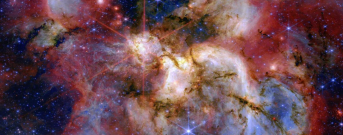
\includegraphics[width=\textwidth]{img/w51_original_panel.png}
        \\[3pt]\small (a) Imagen original
    \end{minipage}
    \hfill
    \begin{minipage}[t]{0.46\textwidth}
        \centering
        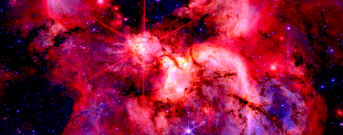
\includegraphics[width=\textwidth]{img/w51_normalizada_panel.png}
        \\[3pt]\small (b) Imagen normalizada
    \end{minipage}
    \caption{Comparación entre la imagen original de W51 y la imagen normalizada tras aplicar la expansión min-max con los rangos R[36--170], G[88--255], B[35--255].}
    \label{fig:comparacion_norm}
    \vspace{2pt}
    {\footnotesize Fuente: Elaboración propia.}
\end{figure}

Tras la normalización, la imagen presenta un contraste notablemente más amplio. Las zonas oscuras del original, que correspondían a regiones de polvo frío donde se encuentran estrellas en formación, comienzan a revelar estructuras antes indiferenciadas. El efecto más evidente se aprecia en los tonos rojos y violáceos que emergen en la imagen normalizada, producto de la expansión de los tres canales de forma independiente. La normalización no crea información nueva: redistribuye las intensidades para que la información ya presente resulte perceptible visualmente.

\subsubsection{Análisis de canales Rojo, Verde y Azul}

La herramienta permite analizar cada canal de color de forma independiente. Para cada canal se muestra su versión original en escala de grises y su versión normalizada, junto con controles deslizantes que permiten ajustar el rango $[p_{\min},\, p_{\max}]$ de forma interactiva. La vista de la interfaz para esta etapa se divide en dos capturas por la extensión de los paneles.

\begin{figure}[!htbp]
    \centering
    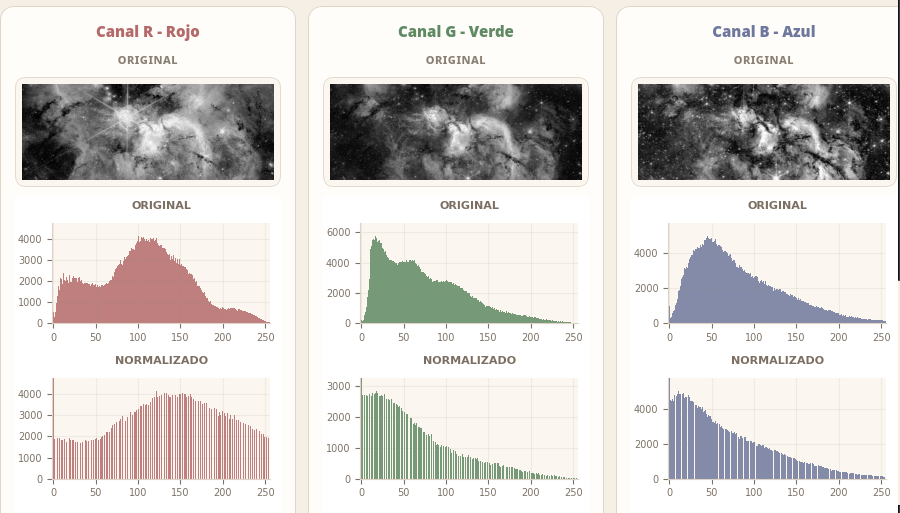
\includegraphics[width=0.92\textwidth]{img/canales_rgb_tarjetas(1).png}
    \caption{Vista superior de las tarjetas de canal: histogramas originales y normalizados del canal R ($p_{\min}=36$, $p_{\max}=170$), G ($p_{\min}=88$, $p_{\max}=255$) y B ($p_{\min}=35$, $p_{\max}=255$) junto con las imágenes originales de cada canal en escala de grises.}
    \label{fig:canales_tarjetas_1}
    \vspace{2pt}
    {\footnotesize Fuente: Elaboración propia.}
\end{figure}

\begin{figure}[!htbp]
    \centering
    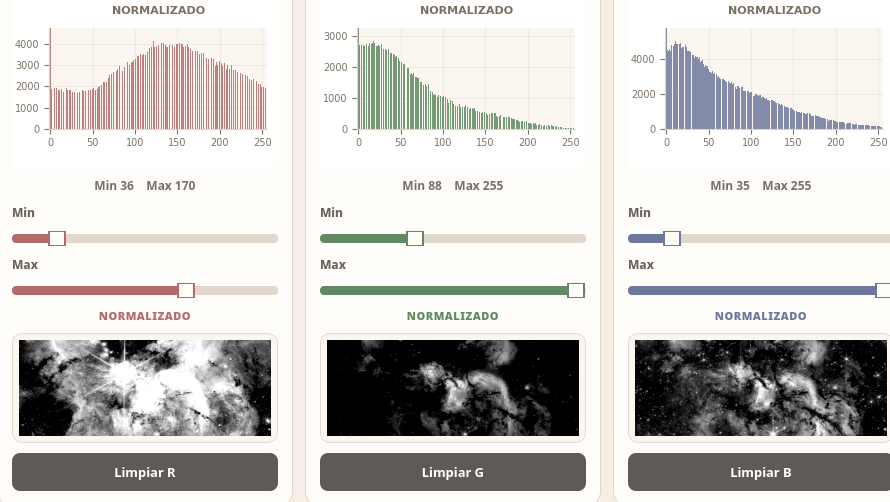
\includegraphics[width=0.92\textwidth]{img/canales_rgb_tarjetas(2).png}
    \caption{Vista inferior de las tarjetas de canal: controles deslizantes de rango e imágenes normalizadas de cada canal (R, G y B), resultantes tras aplicar la expansión min-max con los rangos establecidos.}
    \label{fig:canales_tarjetas_2}
    \vspace{2pt}
    {\footnotesize Fuente: Elaboración propia.}
\end{figure}

\subsubsection{Compresión, escala de grises y binarización}

Tras haber mejorado la visualización mediante la normalización, la segunda pantalla de la herramienta aplica tres transformaciones sucesivas sobre la imagen normalizada: conversión a escala de grises por ponderación de luminosidad, compresión espacial por promediado de bloques y binarización por umbral global \cite{jain}.

La conversión a escala de grises aplica la fórmula de luminosidad ponderada:
\begin{equation}
    I_{gris} = 0.299 \cdot R + 0.587 \cdot G + 0.114 \cdot B
    \label{eq:grises}
\end{equation}
Esta ponderación corresponde al modelo de luminosidad perceptual estándar (Rec.~601) \cite{gonzalez} y es la que implementa la función \texttt{gris\_luma} en \texttt{modelo.py}.

Sobre la imagen en escala de grises se aplica la compresión por bloques: cada región de $N \times N$ píxeles se reemplaza por su valor promedio, lo que reduce la resolución espacial de la imagen y actúa como filtro de suavizado que atenúa el ruido de alta frecuencia sin comprometer los bordes de mayor contraste \cite{szeliski}. La imagen ampliada se genera con \texttt{np.repeat} para mantener las dimensiones originales.

Finalmente, la binarización aplica un umbral global $T$ sobre la imagen comprimida: los píxeles con intensidad mayor o igual a $T$ se convierten en blanco (255) y el resto en negro (0).

\begin{figure}[!htbp]
    \centering
    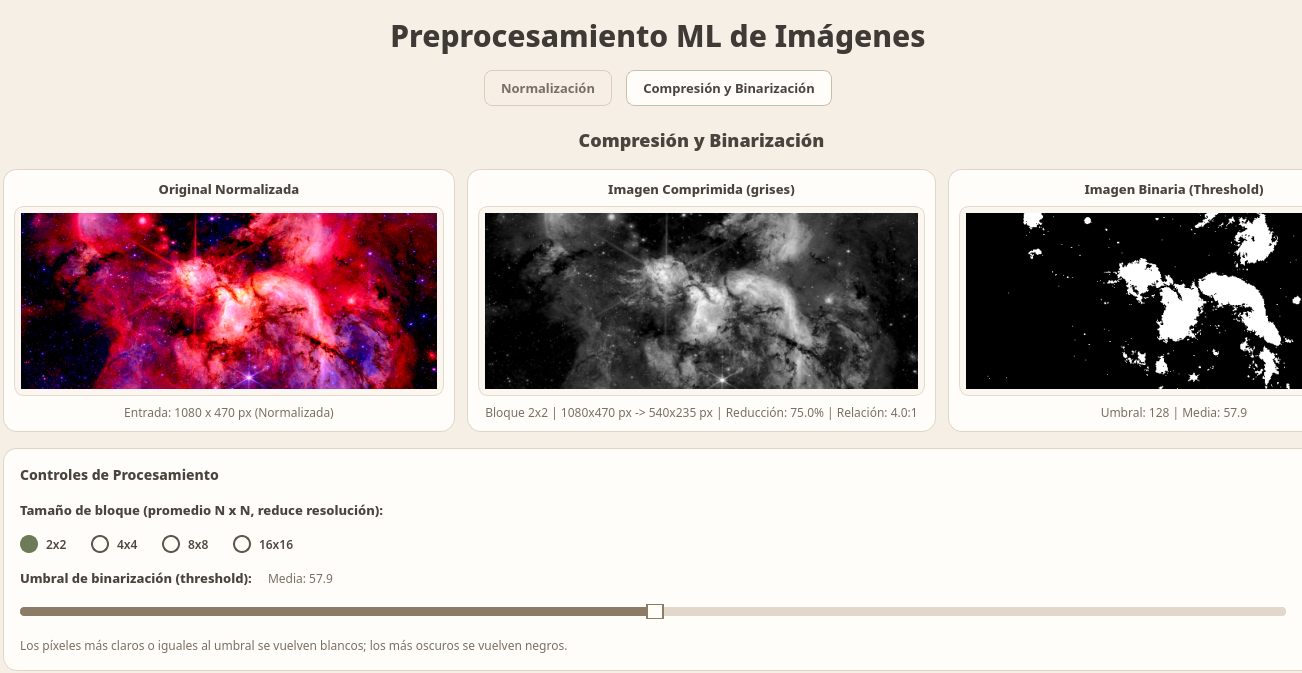
\includegraphics[width=0.92\textwidth]{img/compresion_binarizacion_pantalla.png}
    \caption{Segunda etapa del procesamiento en la herramienta: imagen normalizada de entrada (1080$\times$470 px), imagen comprimida en escala de grises con bloque $2\times2$ (reducción del 75\%, relación 4.0:1) e imagen binaria con umbral $T=128$ sobre una media de 57.9.}
    \label{fig:compresion_binaria}
    \vspace{2pt}
    {\footnotesize Fuente: Elaboración propia.}
\end{figure}

\subsubsection{Controles de procesamiento}

La herramienta expone dos controles interactivos que influyen directamente sobre el resultado:

\medskip
\noindent\textbf{Tamaño de bloque}

Este control define el tamaño $N$ de la región cuadrada que se promedia en la compresión. Las opciones disponibles son $2 \times 2$, $4 \times 4$, $8 \times 8$ y $16 \times 16$. Su comportamiento es el siguiente:
\begin{itemize}
    \item \textbf{$2 \times 2$:} conserva la mayor parte del detalle fino. La simplificación es ligera y las estructuras de menor tamaño se mantienen visibles.
    \item \textbf{$4 \times 4$:} reduce más información y aplica una simplificación intermedia, difuminando gradualmente los detalles más pequeños.
    \item \textbf{$8 \times 8$:} simplifica la imagen en mayor medida; útil para observar patrones generales de brillo, pero los elementos pequeños pierden nitidez.
    \item \textbf{$16 \times 16$:} reduce agresivamente la información fina y puede ocultar estructuras de tamaño reducido, por lo que no es adecuado cuando se busca preservar detalles.
\end{itemize}

\medskip
\noindent\textbf{Umbral de binarización}

Este control, implementado mediante un slider de 0 a 255, establece el valor límite que separa las regiones claras de las oscuras. Un umbral alto restringe la selección a las zonas más brillantes (gas ionizado, estrellas masivas), mientras que un umbral bajo amplía la selección incluyendo regiones de menor intensidad, con el riesgo de incorporar más ruido. La herramienta muestra en tiempo real el valor del umbral seleccionado y el valor de la media de la imagen comprimida como referencia para la selección del umbral.

\begin{figure}[!htbp]
    \centering
    \begin{minipage}[t]{0.46\textwidth}
        \centering
        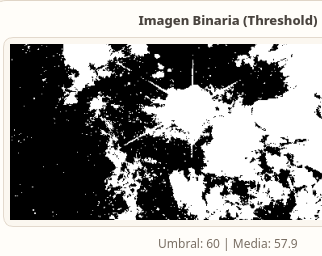
\includegraphics[width=\textwidth]{img/binaria_umbral_bajo.png}
        \\[3pt]\small (a) Umbral bajo ($T \approx 60$): mayor área blanca
    \end{minipage}
    \hfill
    \begin{minipage}[t]{0.46\textwidth}
        \centering
        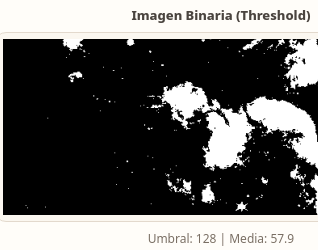
\includegraphics[width=\textwidth]{img/binaria_umbral_128.png}
        \\[3pt]\small (b) Umbral alto ($T = 128$): selección restringida
    \end{minipage}
    \caption{Efecto del umbral de binarización sobre la imagen W51 comprimida (bloque $2\times2$, media = 57.9). Un umbral bajo incrementa el área blanca, mientras que $T=128$ (superior a la media) restringe la selección a regiones de alta intensidad.}
    \label{fig:comparacion_umbrales}
    \vspace{2pt}
    {\footnotesize Fuente: Elaboración propia.}
\end{figure}

\subsubsection{Resultados finales}

Como cierre del procesamiento, se presentan las tres imágenes que resumen el recorrido visual completo: la imagen original de W51, la imagen normalizada y la imagen comprimida en escala de grises. Esta comparación evidencia cómo estructuras poco perceptibles al inicio —estrellas en formación detrás de nubes de polvo— se vuelven visibles después del procesamiento.

\begin{figure}[!htbp]
    \centering
    \begin{minipage}[t]{0.31\textwidth}
        \centering
        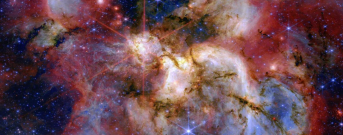
\includegraphics[width=\textwidth]{img/w51_original_panel.png}
        \\[3pt]\small (a) Imagen original
    \end{minipage}
    \hfill
    \begin{minipage}[t]{0.31\textwidth}
        \centering
        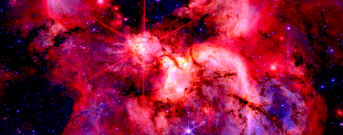
\includegraphics[width=\textwidth]{img/w51_normalizada_panel.png}
        \\[3pt]\small (b) Imagen normalizada
    \end{minipage}
    \hfill
    \begin{minipage}[t]{0.31\textwidth}
        \centering
        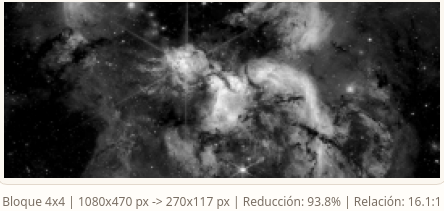
\includegraphics[width=\textwidth]{img/w51_gris_comprimida.png}
        \\[3pt]\small (c) Escala de grises comprimida
    \end{minipage}
    \caption{Resumen visual del flujo completo sobre la imagen W51: (a) imagen original sin procesar, (b) imagen normalizada con expansión min-max por canal R[36--170], G[88--255], B[35--255], y (c) imagen convertida a escala de grises y comprimida con bloque $4\times4$.}
    \label{fig:resultados_finales}
    \vspace{2pt}
    {\footnotesize Fuente: Elaboración propia.}
\end{figure}

\subsection{Habilidades blandas empleadas en la práctica}
$\blacksquare$ Trabajo en equipo \\
$\blacksquare$ Responsabilidad \\
$\blacksquare$ Pensamiento crítico

\subsection{Conclusiones}

La normalización min-max aplicada de forma independiente sobre cada canal RGB permitió ampliar el rango dinámico de la imagen de la región W51, revelando estructuras estelares que en la imagen original permanecían ocultas detrás de las nubes de gas y polvo. El ajuste de los rangos por canal R[36--170], G[88--255], B[35--255] demostró que la selección deliberada de los límites de normalización determina qué información espectral se enfatiza y cuál se descarta.

El análisis por canales RGB evidenció que cada canal aporta información espectral diferente: el canal rojo concentra la emisión general del gas caliente con la distribución más amplia, el canal verde ofrece el mejor contraste entre el polvo frío y el gas ionizado por su menor rango de valores útiles, y el canal azul presenta la distribución más concentrada en intensidades bajas, correspondiente a estructuras de menor temperatura en la región.

La compresión por bloques $N \times N$ aplicada sobre la imagen en escala de grises, seguida de la binarización por umbral global $T$, permitió simplificar la representación de la imagen a dos niveles de intensidad. Con un bloque $2\times2$ y umbral $T=128$ (superior a la media de 57.9), la imagen binaria resultante aísla efectivamente las zonas de mayor brillo —gas ionizado y estrellas masivas— del fondo oscuro de la región.

\subsection{Recomendaciones}

Se recomienda seleccionar imágenes con buena resolución y un histograma que no esté saturado en los extremos, ya que la calidad de la imagen de entrada determina directamente la efectividad de la expansión min-max y la nitidez de los resultados en las etapas de compresión y binarización.

Los rangos mínimo y máximo de cada canal, el tamaño de bloque y el umbral de binarización deben ajustarse considerando las características específicas de la imagen procesada. Un rango demasiado estrecho puede introducir clipping excesivo en los extremos del histograma, mientras que un umbral mal calibrado puede generar una imagen binaria con exceso de ruido o pérdida de estructuras relevantes.

Para trabajos futuros se sugiere incorporar un algoritmo de umbralización adaptativa, como el método de Otsu \cite{opencv_doc}, que calcula automáticamente el umbral óptimo en función de la distribución de intensidades de la imagen comprimida, reduciendo la dependencia del ajuste manual y mejorando la consistencia de los resultados ante imágenes con diferentes características de iluminación.

\subsection{Referencias bibliográficas}
{
    \renewcommand{\refname}{}
    \vspace{-1.5em}

    \begin{thebibliography}{99}
        \bibitem{jwst_w51}
        H.~Yoo and A.~Ginsburg, ``Star formation in W51: First JWST observations,'' University of Florida, Gainesville, FL, USA, 2025. Crédito de imagen: NASA, ESA, CSA, Yoo \& Ginsburg (UF); Procesamiento de imagen: A.~Pagan (STScI). [Online]. Available: \texttt{https://www.nasa.gov/missions/webb/}

        \bibitem{gonzalez}
        R. C. Gonzalez and R. E. Woods, \textit{Digital Image Processing}, 4th ed. New York, NY, USA: Pearson, 2018.

        \bibitem{jain}
        A. K. Jain, \textit{Fundamentals of Digital Image Processing}. Englewood Cliffs, NJ, USA: Prentice Hall, 1989.

        \bibitem{szeliski}
        R. Szeliski, \textit{Computer Vision: Algorithms and Applications}, 2nd ed. Cham, Switzerland: Springer, 2022.

        \bibitem{opencv_doc}
        OpenCV Team, ``Image Thresholding,'' in \textit{OpenCV Documentation}, version 4.x. [Online]. Available: \texttt{https://docs.opencv.org/4.x/d7/d4d/tutorial\_py\_thresholding.html}
    \end{thebibliography}
}

\end{document}
